\begin{IEEEbiography}[{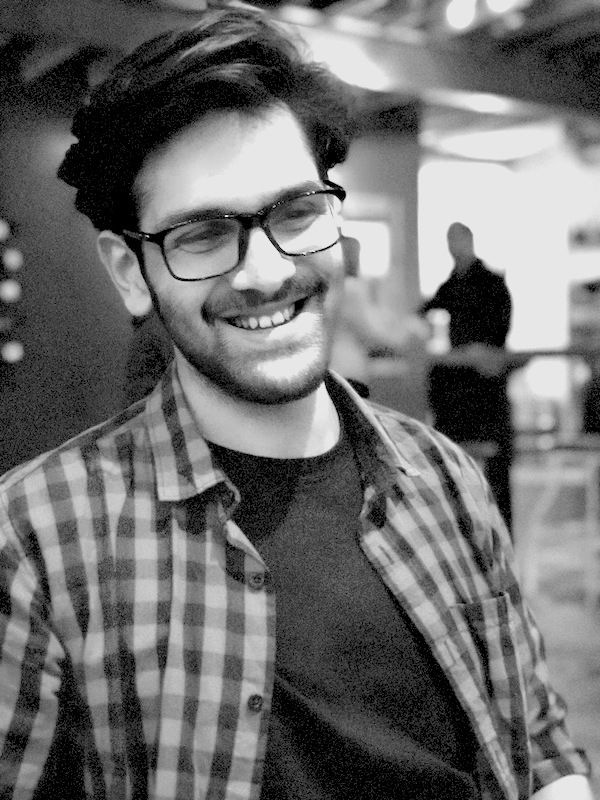
\includegraphics[width=1in,height=1.3in,clip]{images/rahul.png}}]
{Rahul Krishna} is a Ph.D. student in the department of Computer Science at NC State University. He received his master's degree in Electrical Engineering also at NC State University. His interest lies in exploring ways in which artificial intelligence can be used to generate actionable analytics for software engineering. He currently works on developing machine learning algorithms that go beyond prediction to assist in decision making. For more information, visit \url{http://rkrsn.us}.
\end{IEEEbiography}
\begin{IEEEbiography}[{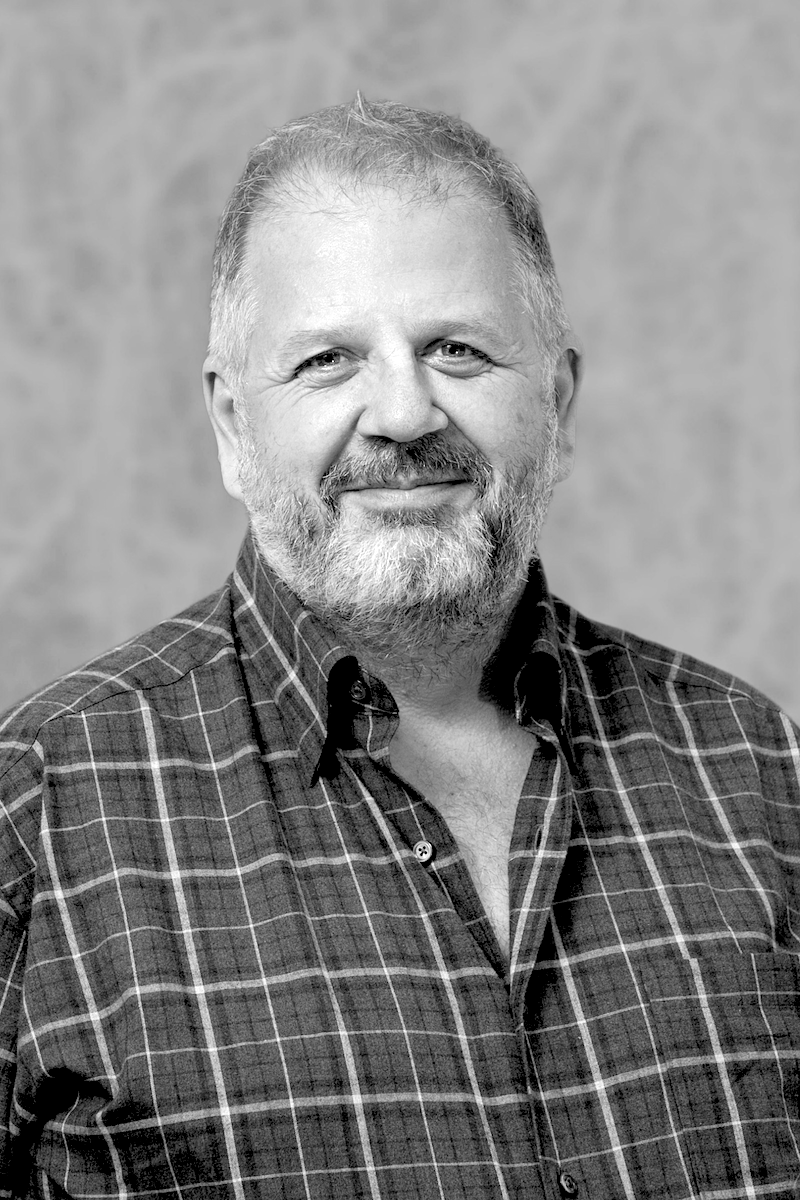
\includegraphics[width=1in, height=1.3in, clip]{images/tim.png}}]
{Tim Menzies} (Ph.D., UNSW, 1995) is a full Professor in CS at NC State University, where he explores SE, data mining, AI, search-based SE, and open access science. He is the author of over 250 referred publications and co-founder of the PROMISE conference series devoted to reproducible experiments in SE (\url{http://tiny.cc/seacraft}).  Dr. Menzies also serves as associated editor of many journals:  IEEE TSE, ACM TOSEM, Empirical Software Engineering, ASE Journal, Information Software Technology, IEEE Software, and the Software Quality Journal. For more, see \url{http://menzies.us}.
\end{IEEEbiography}